\documentclass [handout] {beamer}

\usepackage{graphicx, subfigure}
\usepackage{amsmath}


% \usepackage{beamerthemesplit} // Activate for custom appearance


\title{\color{blue}Missing Value Imputation using Low-Rank and Low-Norm Models}
\subtitle{\color{magenta}Knowledge Lab Team Presentation}
\author{ Nandana Sengupta \\ (co-authored with James Evans and Madeleine Udell)}
\date{\color{blue}\today}

\begin{document}

\frame{\titlepage}

\frame{
\frametitle{Introduction}
\begin{itemize}
\item<2-> Missing data arise in almost all empirical analysis.
\item<3-> Distracts from main goal of study.
\item<4-> \color{magenta} Ad-hoc methods \color{black} 
\begin{itemize}
\item<5-> Complete case analysis.
\item<6-> Available case analysis. 
\item<7-> Mean Imputation.
\end{itemize}
\item<8-> Concerns about validity of inferences.
\item<9-> \color{magenta}Types of Missing Data \color{black}
\begin{itemize}
\item<10-> Missing Completely at Random.
\item<11-> Missing at Random.
\item<12-> Missingness depends on unobservables.
\end{itemize}



\end{itemize}


}




\frame{
\frametitle{Multiple Imputation}
\begin{itemize} \small
\item<2-> Rubin (1976), Schafer (1998), Van Buuren et al (1999), King et al (2000, 2015)
\item<3-> \color{magenta}Idea: \color{black} Analysis should reflect uncertainty inherent in imputation.
\item<4-> \color{magenta} Assumption: \color{black}MAR
\item<5-> 3 stage scheme
\begin{itemize}
\item<6-> \color{magenta} Imputation \color{black}
\item<7-> \color{magenta} Analysis \color{black}
\item<8-> \color{magenta} Combining Results\color{black}
\end{itemize}
\item<9-> Imputation Step:
\begin{itemize}
\item<10-> Parametric Assumptions (like multivariate normality).
\item<11-> Iterative procedures used.
\end{itemize}
\end{itemize}
}


\frame{ \frametitle{Multiple Imputation}
\begin{itemize} \small
\item<2-> \color{magenta} Two Standard Imputation Approaches:
\begin{itemize}
\item<3-> MCMC mechanism:  $(Y^{(1)}_{miss}, \theta^{(1)} ), (Y^{(2)}_{miss}, \theta^{(2)} ), \ldots$.
\item<4-> Chained Equations: iteratively fit univariate regression models.
\end{itemize}
\item<5-> \color{magenta} Analysis: \color{black} perform as if full data is observed.
\item<6->\color{magenta} Combining Results:
\begin{itemize} \small
\item<7-> \color{magenta}Point Estimate: \color{black} $ \overline{Q} = \frac{1}{m}  \sum \limits_{i = 1}^m \widehat{Q_i}  \quad; \widehat{Q_i} =$ point estimate from imputation $i$.  
\item<8->  \color{magenta} Variance: \color{black} $T = \overline{U} + \left( 1+ \frac{1}{m}\right) B \quad$;  $U=$ within imputation variance ; $B=$ between imputation variance. 
\end{itemize}
\item<9-> `R' Packages: Amelia, MICE, MI.
\end{itemize}
}


\frame{
\frametitle{Low Norm and Low Rank Models}
\begin{itemize} \small
\item<2-> Matrix Factorization approaches.
\item<3-> Srebro (2004), Udell et al (2014).
\item<4-> Approximate matrix $A$ ( dimension $m \times n$) by $X'Y$. 
\item<5-> minimize \color{magenta}$ \sum_{i,j} L_{i,j} (x_i y_j, a_{ij}) + \sum \limits_{i=1}^{m} r_i(x_i) + \sum \limits_{j=1}^{n} r_j(y_j)   $.
\begin{itemize}
\item<6-> $L$: Loss function (over columns).
\item<7-> $r(.)$ : regularization functions.
\item<8-> $X$, $Y$ initialization: SVD good starting point.
\item<9-> \color{magenta} Low Norm Models: \color{black} $r(x) = \gamma ||X^2||$.
\item<10-> \color{magenta} Low Rank Models: \color{black} $Rank(X'Y) \leq k$.  
\item<11-> \color{magenta} Low Rank, Low Norm Models: \color{black} Both
\item<12-> $k$, $\gamma$ chosen via crossvalidation.
\end{itemize}
\item<13-> Julia Implementation: LowRankModels 
\end{itemize}
}





\frame{
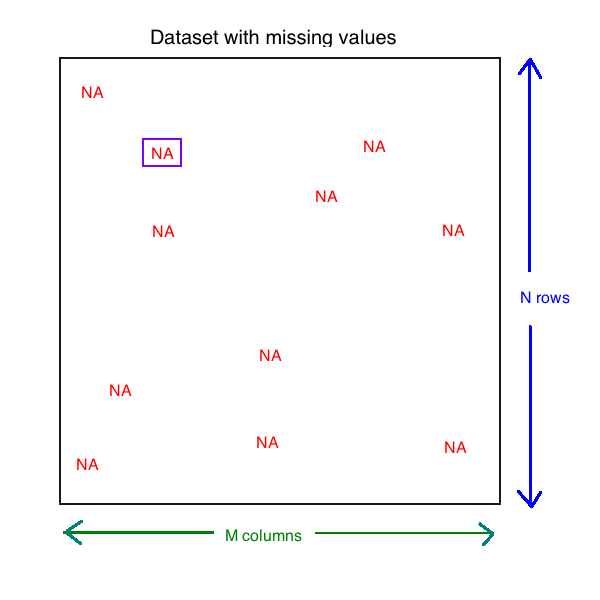
\includegraphics[width =0.85 \textwidth]{fig1}

}


\frame{
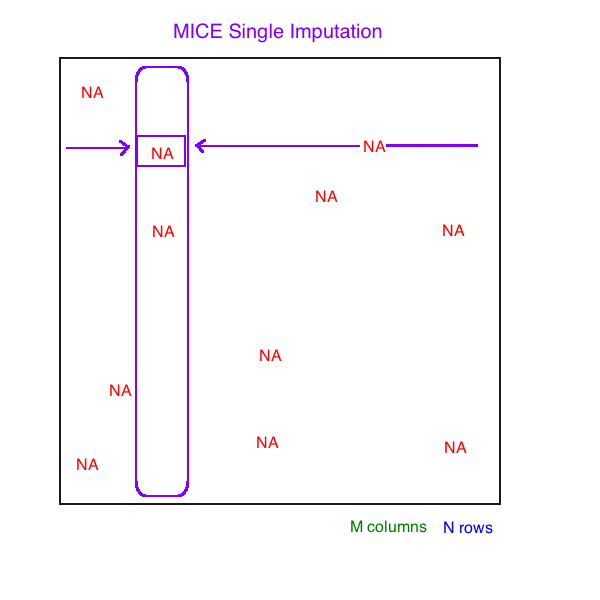
\includegraphics[width = 0.85\textwidth]{fig2}
}


\frame{
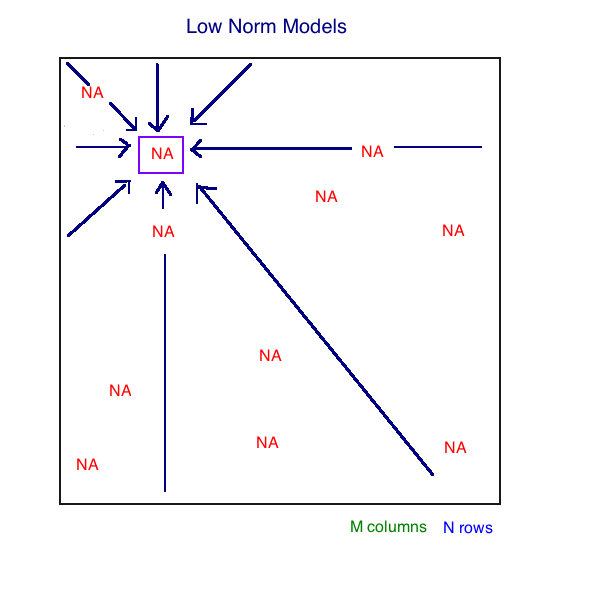
\includegraphics[width = 0.85\textwidth]{fig4}
}

\frame{
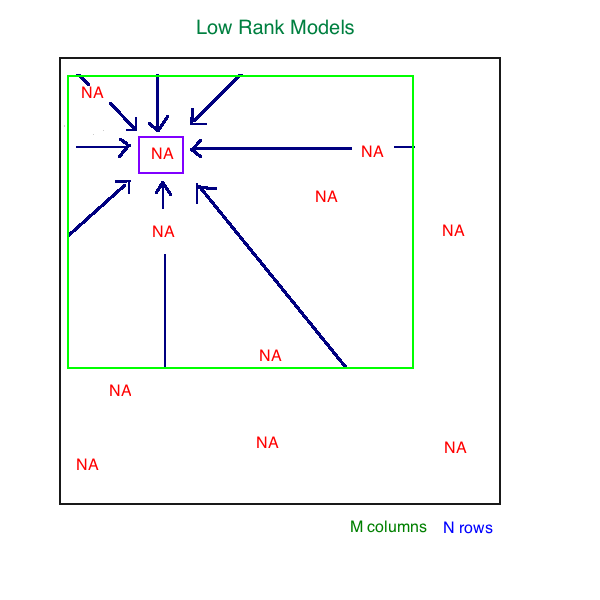
\includegraphics[width = 0.85\textwidth]{fig3}
}




\frame{
\frametitle{Application 1: General Social Survey Data (GSS)}
\begin{itemize}\small
\item<2->  Sociological survey: adults in randomly selected US households.
\item<3->  Data on attitudes and demographic characteristics of adults.
\item<4-> \color{magenta}Subset of GSS 2014 data used for analysis
\begin{itemize}\small
\item<5-> columns corresponding to identifying variables
\item<6-> columns with non-varying entries
\item<7-> $ \geq 33 \%$ missing entries
\item<8-> highly correlated columns ($\rho > 0.70$).
\end{itemize}
\item<9-> \color{magenta}Evaluation Strategy 
\begin{itemize}\small
\item<10->  $10 \%$ of observed data are randomly assumed missing ($N_{miss,ind}$)
\item<11-> Imputations using
\begin{itemize} \small
\item<12->\color{magenta} Low Rank (Scaled), Low Rank (Unscaled), Trace Norm (Full Rank), Trace Norm (Low Rank), MICE.
\end{itemize}
\item<13-> Loss calculated over $N_{miss,ind}$ observations: 
\begin{itemize} \small
\item<14-> \color{magenta} scale columns, quadratic loss over non-categorical columns, zero-one loss over categorical columns. 
\end{itemize}
\end{itemize}
\end{itemize}
}

\frame{
\frametitle{Results}
\begin{itemize} \small
\item<2-> \small Overall Trace (Full Rank) had lowest loss, all Low Rank and Low Norm models outperformed MICE
\item<3-> \small Column-wise: $\approx  80\%$ columns had lower loss compared to MICE


\item<4-> \color{magenta} \centering \small{Summary Table}
 \color{black}
% Wed Sep  9 16:27:42 2015
\begin{table}[H] \tiny
\centering
\begin{tabular}{|c|c|c|c|c|c|} 
  \hline
 & LowRank (S) & LowRank (NS) & Trace (FR) & Trace (LR) & MICE \\ 
  \hline
Scaled Loss/($10^3$) & 18.50 & 15.80 & 14.40 & 15.80 & 20.60 \\ 
  \%age reduction over MICE& 10.10   \%& 23.40  \% & 30.10  \% & 23.00  \% & -- \\ 
  \%age cols w/ lower loss & 73.50   \% & 84.60   \% & 87.20   \% & 84.60  \% & -- \\ 
   \hline
\end{tabular}
\end{table}
\item<5-> 
\begin{center} \color{magenta}  \small{Columnwise percentage reduction in Loss over MICE} \end{center}
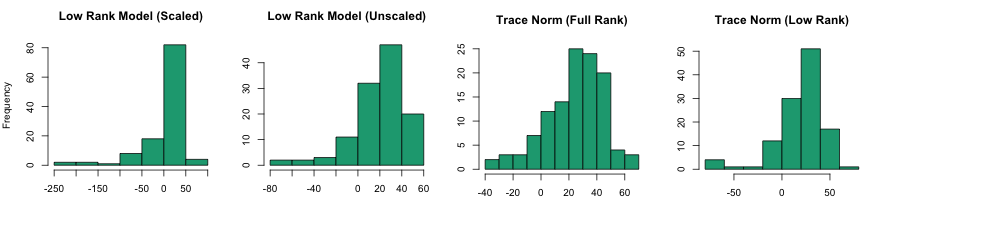
\includegraphics[width = 1.125\textwidth]{percent_gss}
\end{itemize} 
}


\frame{
\frametitle{Results}

\begin{itemize}

\item<2-> 
\begin{center} \color{magenta}  \small{Method with  lowest loss across columns  } \end{center}
\begin{center}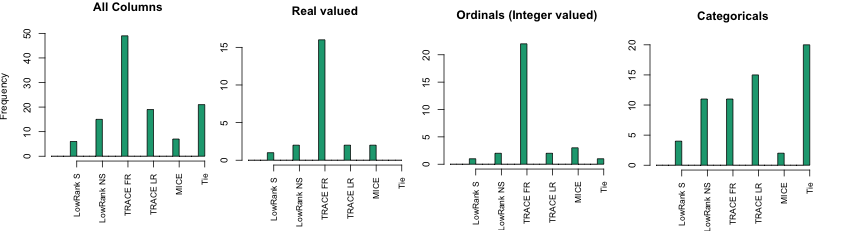
\includegraphics[width = 1.05\textwidth]{select_gss} \end{center}


\item<3-> 
\begin{center} \color{magenta}  \small{Categorical columns misclassification by method} \end{center}
\begin{center} 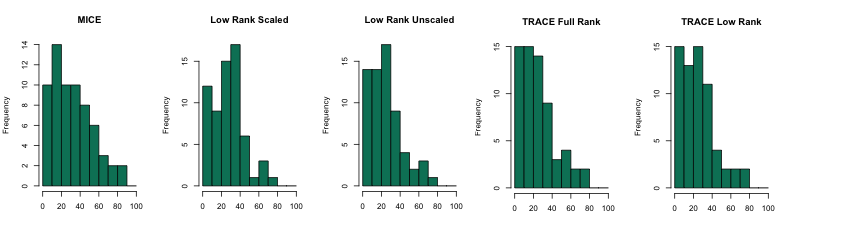
\includegraphics[width = 1.1\textwidth]{categoricals_gss} \end{center}
\end{itemize} 


}






\frame{ 
\frametitle{Next Steps}
\begin{itemize} \small
\item<1-> Replicating missingness patterns before applying imputation techniques.
\item<2-> Extending and applying to longitudnal survey data (e.g. National Longitudnal Survey of Youth).
\item<3-> Applying to larger subsets of GSS data.
\item<4-> Working with more advanced options of MICE and LowRankModels.
\item<5-> Extending to Max and Frobenius norms.
\item<6-> Extending Low Rank and Low Norm methods to Multiple Imputation setting. 
\end{itemize}
}





\frame{
\begin{block}{}
\color{magenta}Thank you!
\\(Comments and Suggestions Welcome)
\end{block}}

\end{document}




\frame{
\frametitle{Application 2: Simulated Dataset}

}

\frame{
\frametitle{Results}


}


\frame{
\frametitle{Results}


}